\documentclass[11pt]{article}
\usepackage[utf8]{inputenc} % Para caracteres en espa�ol
\usepackage{amsmath,amsthm,amsfonts,amssymb,amscd}
\usepackage{multirow,booktabs}
\usepackage[table]{xcolor}
\usepackage{fullpage}
\usepackage{lastpage}
\usepackage{enumitem}
\usepackage{multicol}
\usepackage{fancyhdr}
\usepackage{mathrsfs}
\usepackage{wrapfig}
\usepackage[final]{pdfpages}
\usepackage{setspace}
\usepackage{esvect}
\usepackage{calc}
\usepackage{multicol}
\usepackage{cancel}
\usepackage{graphicx}
\graphicspath{ {pictures/} }
\usepackage[retainorgcmds]{IEEEtrantools}
\usepackage[margin=3cm]{geometry}
\usepackage{amsmath}
\newlength{\tabcont}
\setlength{\parindent}{0.0in}
\setlength{\parskip}{0.05in}
\usepackage{empheq}
\usepackage{framed}
%\usepackage{newtxmath}
\usepackage{euscript}
\DeclareMathAlphabet{\mathpzc}{T1}{pzc}{m}{it}
\usepackage[most]{tcolorbox}
\usepackage{xcolor}
\colorlet{shadecolor}{orange!15}
\parindent 0in
\parskip 12pt
\geometry{margin=1in, headsep=0.25in}
\theoremstyle{definition}
\newtheorem{defn}{Definition}
\newtheorem{reg}{Rule}
\newtheorem{exer}{Exercise}
\newtheorem{note}{Note}
\newcommand{\volume}{{\ooalign{\hfil$V$\hfil\cr\kern0.08em--\hfil\cr}}}
\newcommand{\parr}{\mathbin{\|}} % Parralel Symbol
\begin{document}
\setcounter{section}{1}%Section we want -1
\setcounter{page}{22} %Page we want
\setcounter{equation}{33}%Equation we want -1
\def\thepart{\arabic{part}}
\setcounter{part}{8}
\numberwithin{equation}{part}

 \pagestyle{fancy}
\fancyhf{}
\rhead{Section 8:  Electromagnetic Propulsion - Particle Description}
\rfoot{Page \thepage}
\thispagestyle{empty}

\begin{center}
{\LARGE \bf Section 8:  Electromagnetic Propulsion}\\
{\large AE435}\\
Spring 2018
\end{center}
\vspace{5mm}
\section{Particle Description}
\vspace{25mm}
\tableofcontents
\newpage
In the particle description the MPD acts like an ion thruster but with a neutral plasma.  Ions are driven from the anode and electrons from the cathode.  Particles are collisionless.


 \begin{center}
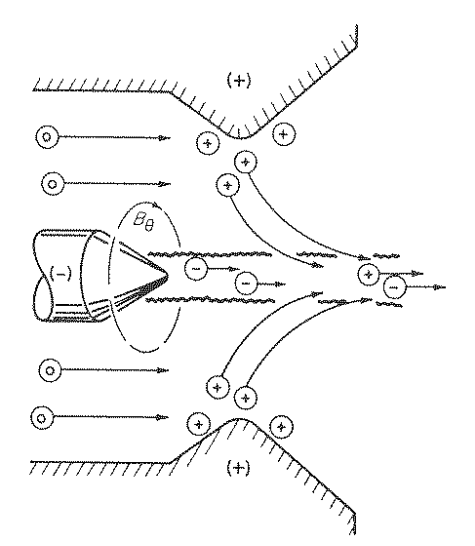
\includegraphics[scale=0.6]{PD.png} 
\end{center}

Note as ions approach the cathode, 3 things happen:
\begin{enumerate}
\item Ions are accelerated by $E_r$ inward gaining velocity.
\item $B_{\theta} \sim \frac{1}{r}$  so $r_L$ gets smaller as $B_{\theta}$ increases. As they move inward, $B_{\theta}$ has more of an influence on them causing them to bend (v x B), do gyro motion.
\item Ions are turned axially
\end{enumerate}
$r_L$ is Larmor radius
 \begin{equation*}
 \begin{aligned}
 r_L = \frac{m \, v_{\perp}}{|q| \, B}
 \end{aligned}
 \end{equation*}
 
Current and mass flow related by:
  \begin{equation}
 \begin{aligned}
 J = \frac{\dot{m} \, e}{M}
 \end{aligned}
 \end{equation}
 
For singly-ionized particles with M being the mass of ions.
 
Using Equation 8.18, $ B = \frac{\mu_o \, J}{2 \, \pi \, r}$, and Equation 3.11, $r_L = \frac{M \, v_+}{e \, B}$ (mass of ion, velocity of ion): it can be said that the $r_L$ must be smaller than radius, in other words,
 
  \begin{equation}
 \begin{aligned}
 r \ge r_l = \frac{M \, v_+}{e \, B} = \frac{2 \, \pi \, r \, M \, v_+}{e \, \mu_o \, J}
 \end{aligned}
 \end{equation}
 
 Looking at this from a particle point of view, we are going to find a limit on the current or how the current scales. 
 
If we replace $v_+$ with $u_e$ (fluid exit velocity, speed of ions as they leave the MPD), we can write a requirement on J, which will be large enough to turn ions if:
 
  \begin{equation}
 \begin{aligned}
 J > \frac{2 \, \pi \, M \, u_e}{e \, \mu_o}
 \end{aligned}
 \end{equation}
 
 Where 
 
  \begin{equation*}
 \begin{aligned}
 M &= A \, m_{\text{proton}} \\ \\
 A &= \text{Atomic Weight} \\ \\
 m_{\text{proton}} &= 1.6726219 \times 10^{-27} \, [kg] \\
 &= 0.992776097 \, [amu]
 \end{aligned}
 \end{equation*}
 
 such that
 
  \begin{equation*}
 \begin{aligned}
  J > \frac{2 \, \pi \, m_{\text{proton}}}{e \, \mu_o} \, A\,u_e = 0.0522 \, A \, u_e \sim \frac{A \, u_e}{20}
 \end{aligned}
 \end{equation*}
 
 If we want higher specific impulse, we want smaller mass ions and larger current. 
 \newpage
 \begin{framed} 
\textbf{Example: } Consider an Argon particle with atomic mass, A = 40 [amu] with an exit velocity $u_e = 40,000 \, [m/s]$. We want the resulting current to be greater than 80 kA, $J > 80 \, [kA]$. 

We are looking at the scaling of a current from a scaling point of view.
 
In practice this current level is higher than is actually used.  But the relation does illustrate two points:
\begin{enumerate}
\item Current and ion mass, M, are coupled
\item Since J is limited for practical reasons (higher current means higher mass power electronics, high current switching, etc.), lighter ions have higher $I_{SP}$
\end{enumerate}
 
Current and mass flow rate are coupled (Equation. 8.34), so
 
  \begin{equation*}
 \begin{aligned}
 J \sim \frac{A \, u_e}{20} = \frac{e \, \dot{m}}{A \, m_{\text{proton}}} \quad \rightarrow \quad \dot{m} \cong \frac{1}{20} \, \frac{m_{\text{proton}}}{e} \, A^2 \, u_e
 \end{aligned}
 \end{equation*}
 Thus
 
  \begin{equation*}
 \begin{aligned}
 F = \dot{m} \, u_e =  \frac{m_{\text{proton}}}{20 \, e} \, A^2 \, u_e^2
 \end{aligned}
 \end{equation*}
 
  \begin{equation*}
 \begin{aligned}
 Z = \frac{1}{2}\, k \, u_e \quad \rightarrow \quad V = Z \, J = \frac{1}{2}\, k \, u_e \, J =  \frac{1}{2}\, k \, u_e \, \frac{A \, u_e}{20}
 \end{aligned}
 \end{equation*}
 
  \begin{equation*}
 \begin{aligned}
 V = \frac{k \, A \, u_e^2}{40}
 \end{aligned}
 \end{equation*}

 \end{framed}
 \newpage
\subsection{The mass injection problem}
It was found that performance was improved by mass injection at large radius.  Performance depends on where the ions are produced.  Larger radius is better cause get more energy from $E_r$. For the ions to build up as much energy, you will have to have it start at a large radius away from the cathode that way it can accelerate towards it for a longer period of time. In general, you want the mass injection to be along the outer radius such that the ions can be created close to the anode surface.
 \begin{center}
 \vspace{70mm}
 \textbf{Figure 1}
 \end{center}
 
 
 
 
 

 
 
 
 
 
 
 
 
 
 
 
 
 
 
 
 
 
 
 
 
 
 


\end{document}